\documentclass[conference]{IEEEtran}
\IEEEoverridecommandlockouts
% The preceding line is only needed to identify funding in the first footnote. If that is unneeded, please comment it out.
\usepackage{cite}
\usepackage{amsmath,amssymb,amsfonts}
\usepackage{algorithmic}
\usepackage{graphicx}
\usepackage{textcomp}
\usepackage{xcolor}
%\usepackage{booktabs}
\usepackage{tabularray}
\UseTblrLibrary{booktabs}
\def\BibTeX{{\rm B\kern-.05em{\sc i\kern-.025em b}\kern-.08em
    T\kern-.1667em\lower.7ex\hbox{E}\kern-.125emX}}
\begin{document}

\title{Evaluation of a genetic algorithm based image approximation method}

\author{\IEEEauthorblockN{Gergely Vakulya}
\IEEEauthorblockA{\small \textit{Alba Regia Technical Faculty} \\
\textit{Óbuda University}\\
\textit{Székesfehérvár, Hungary}\\
\textit{vakulya.gergely@amk.uni-obuda.hu}
}}

\maketitle

\begin{abstract}
In this paper
\end{abstract}

\begin{IEEEkeywords}
genetic algorithm, image approximation
\end{IEEEkeywords}

\section{Introduction}

Genetic algirithms (GA) \cite{ga-book} offer good approximations to many
problems, where no fast algorithm is known to calculate
the optimal solutions. It models the natural selection,
where each member of a population (called specimen)
represents one possible solution.

GA starts with an initial population, which is a set of
possible solutions (e.g. empty or randomly generated).
In each cycle GA produces new specimens by applying
\emph{mutation} and \emph{crossover} operations on the
existing ones. Then the population is evaluated by
the \emph{selection} operator based on the \emph{fitness}
function.

In this paper a GA-based lossy image compression method is
presented. A number of triangles are used to approximate
a monochromatic image; the position of the triangles are
optimized with GA. The chromosome representation, the
mutation nad crossover operators and different selection
strategies are evaluated. The algorithm is capable to give
recognizable approximation of images in the 100 byte range.

\section{Previous work}

Genetic algorithms are suitable to problems, where
there no efficient solution is available to calculate
the optimal (or, in many cases, any) solution.
An advantage of GA is the iterative operation, making it possible
to stop the optimization process in any time and use the current
best solution.

Scheduling is an everyday problem in industy \cite{ga-scheduling}
and transportation planning \cite{ga-transport}, where genetic
algorithms can offer a good alternative to e.g. linear programming.

A good application of genetic algorithm is calculating
the synaptic weights of neural networks. MarIO \cite{mar-io}
is an AI player to the Super Mario game.

Genetic algorithms are also suitable to generate program code
(genetic programming) to determine the behavior of e.g.
autonomous robots. A good example is \cite{ga-robocode},
where a specialla tailored programming language (Robocode)
is used to program virtual battle robots.

In economics portfolio optimization \cite{ga-portfolio}
and automatic trading \cite{ga-trading}
can be implemented with genetic algorithms.

\cite{image-proc}

\section{The GA-based image compression}

\subsection{Problem statement}

An image $IMG$ is given as square ($n \times n$) matrix, where each pixel is
either black or white:

\begin{equation}
	IMG = (a_{ij}) \in {0,1}^{n \times n}
\end{equation}

An approximation is given as a set of $n$ triangles. The corner points of
the triangles are placed in the target image, in integer positions,
and can have either black or white color. The $k^\text{th}$ triangle
$t_k$ can be given as a quad:

\begin{equation}
	t_k = (A, B, C, c), A, B, C \in {1 \dots n}^2, c \in {0, 1}
\end{equation}

Time $I(t_k)$ image of triangle $t_k$ is a set of points, which are geometrically
between the corners:

\begin{equation}
	\begin{split}
	I(t_k) &= {a_{ij}},\\
	\exists \alpha, \beta &\in [0, 1]:\\
	i &= \beta(\alpha A_1 + (1-\alpha)B_1)+(1-\beta)C_1\\
	j &= \beta(\alpha A_2 + (1-\alpha)B_2)+(1-\beta)C_2
	\end{split}
\end{equation}

\subsection{Chromosome representation}

The chromosome representation is a tripe $(k, T, C)$, where

\begin{itemize}

	\item{$k \in Z$ is the number of triangles used in the approximation,}

	\item{$T \in Z^{k \times 3 \times 2}$ is the set of triangles, given with 3 coordinate pairs,}

	\item{$C \in {0,1}^k$ is the set of triangle colors.}

\end{itemize}

\subsection{Fitness function}

Instead of the fitness function, where the more suitable
specimen have larger fitness, an $E$ error function is used, representing
the mismatching area between the target image and the triangle
based approximation.

\begin{equation}
	E = \sum_{i,j} \left( \frac{IMG_{ij}-A_{ij}}{mn} \right), 1 \leq i \leq n, 1 \leq j \leq n
\end{equation}

\subsection{Genetic operators}

\subsection{Software architecture}

The image approximation algorithm is implemented in C,
without using external libraries (besides glibc). This
approach makes the code easily portable, but on the other
hand it makes handling of different image formats more
difficult. Thus, only loading and saving of BMP files
with predefined resolution and color depth are supported.

\section{Test results}

\subsection{Test images}

\begin{figure}[htbp]
	\centering
	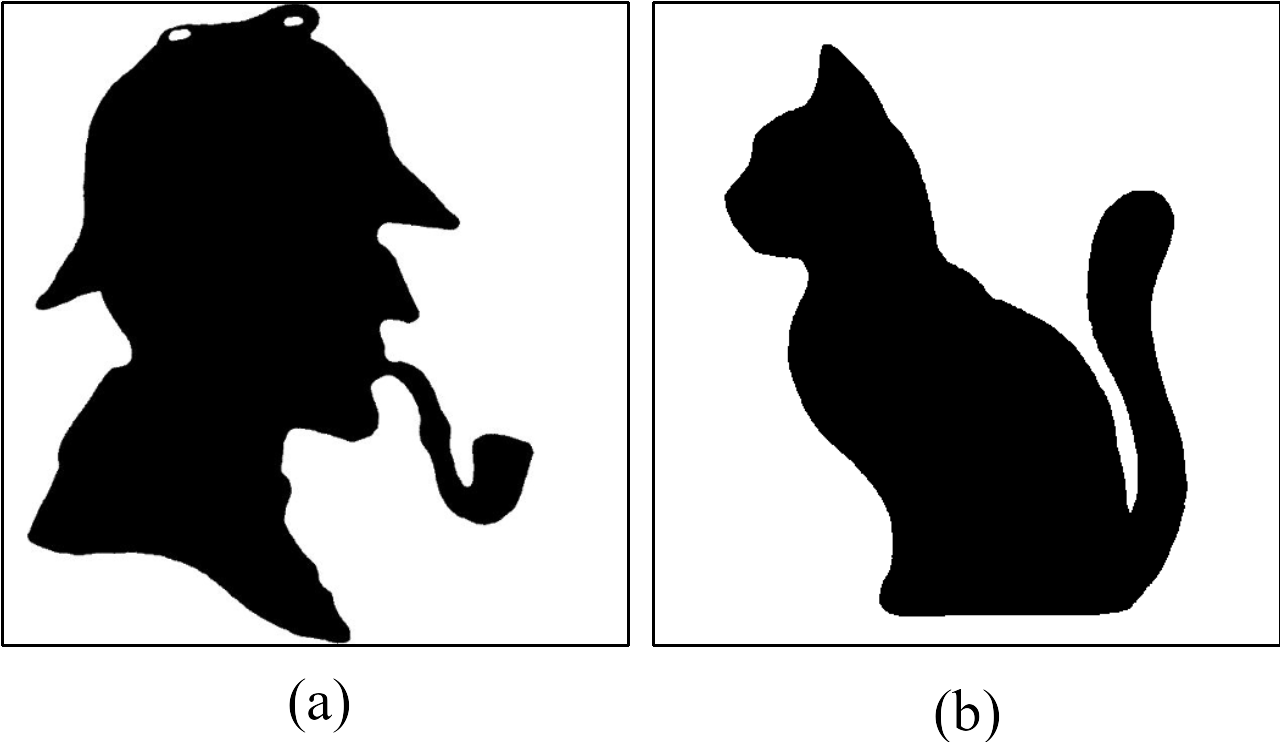
\includegraphics[width=0.35\textwidth]{fig/originals.png}
	\caption{The selected test images. (a) Silhouette of Sherlock Holmes, (b) Silhouette of a cat.}
	\label{fig-orig}
\end{figure}

\begin{figure}[htbp]
	\centering
	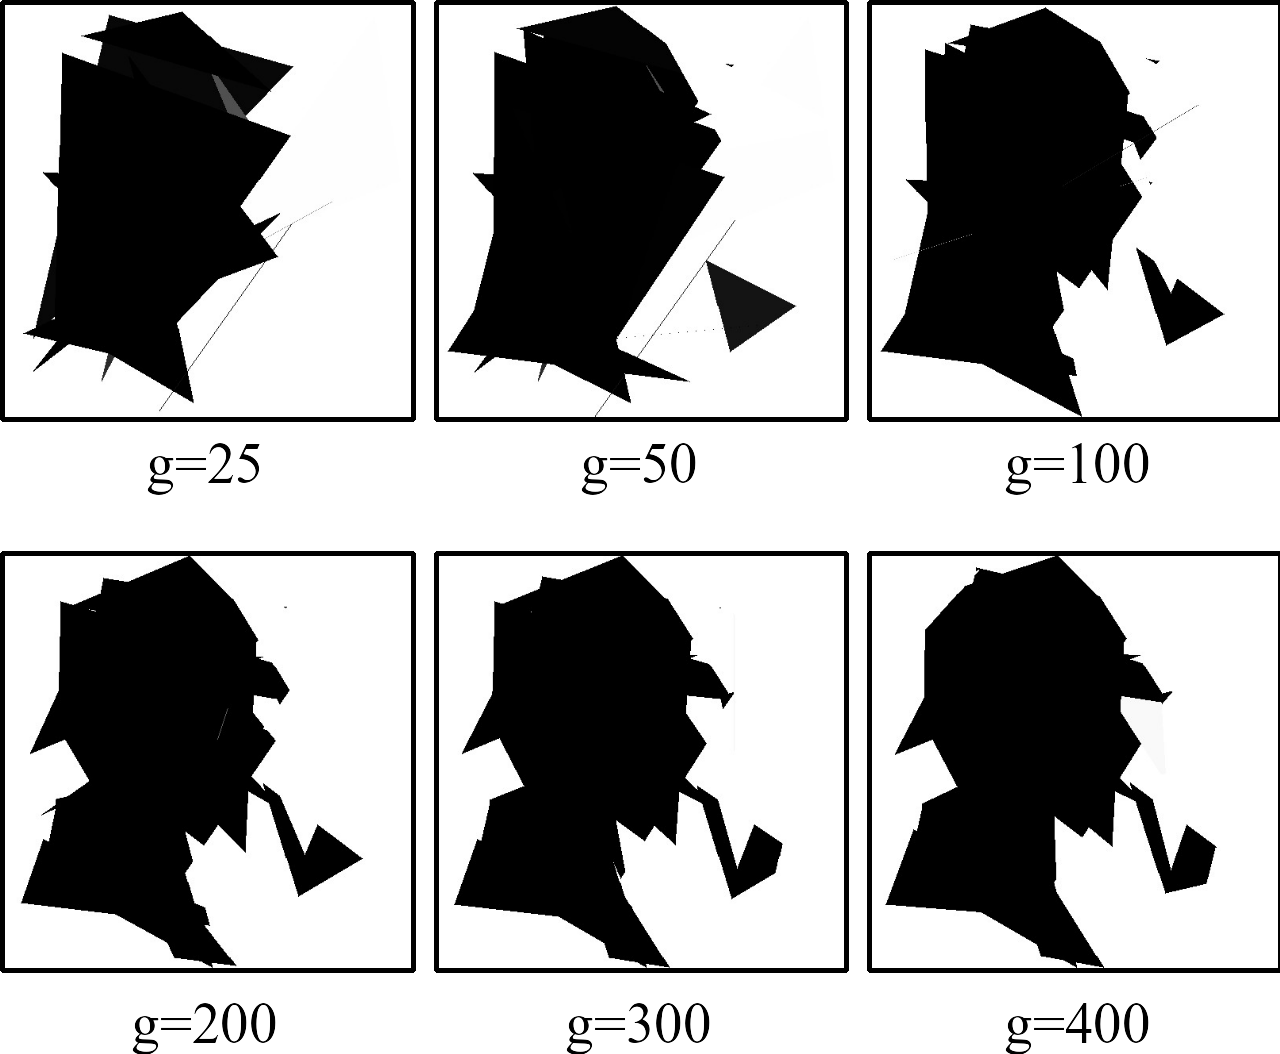
\includegraphics[width=0.35\textwidth]{fig/sherlock6.png}
	\caption{The best matching Sherlock image after $g$ generations.}
	\label{sherlock-6}
\end{figure}

\begin{figure}[htbp]
	\centering
	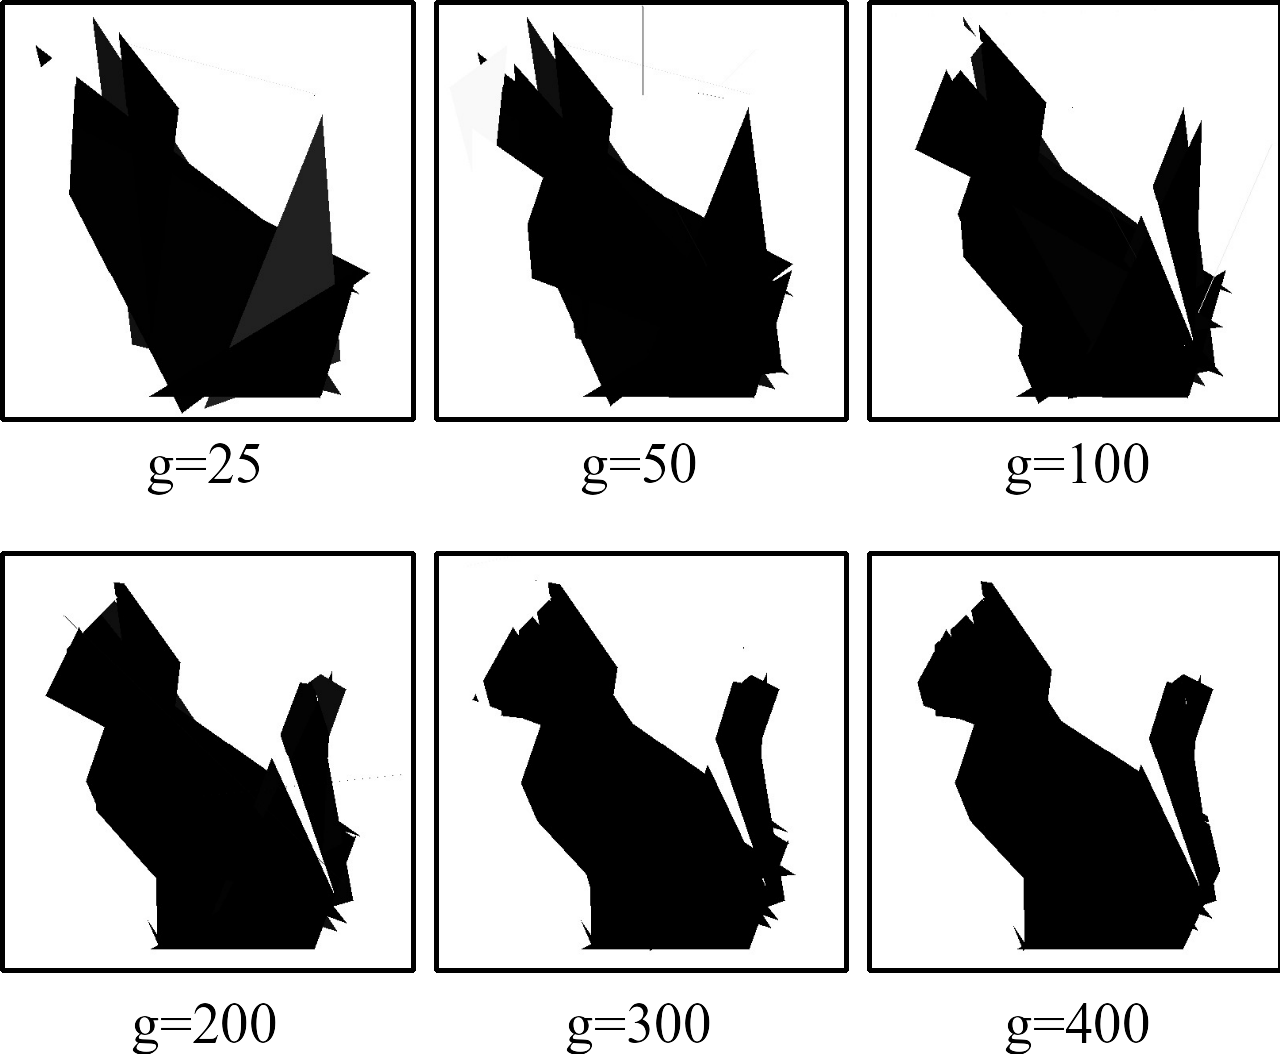
\includegraphics[width=0.35\textwidth]{fig/cat6.png}
	\caption{The best matching cat image after $g$ generations.}
	\label{cat-6}
\end{figure}


\begin{figure}[htbp]
	\centering
		\resizebox{.45\textwidth}{!}{% GNUPLOT: LaTeX picture with Postscript
\begingroup
  \makeatletter
  \providecommand\color[2][]{%
    \GenericError{(gnuplot) \space\space\space\@spaces}{%
      Package color not loaded in conjunction with
      terminal option `colourtext'%
    }{See the gnuplot documentation for explanation.%
    }{Either use 'blacktext' in gnuplot or load the package
      color.sty in LaTeX.}%
    \renewcommand\color[2][]{}%
  }%
  \providecommand\includegraphics[2][]{%
    \GenericError{(gnuplot) \space\space\space\@spaces}{%
      Package graphicx or graphics not loaded%
    }{See the gnuplot documentation for explanation.%
    }{The gnuplot epslatex terminal needs graphicx.sty or graphics.sty.}%
    \renewcommand\includegraphics[2][]{}%
  }%
  \providecommand\rotatebox[2]{#2}%
  \@ifundefined{ifGPcolor}{%
    \newif\ifGPcolor
    \GPcolortrue
  }{}%
  \@ifundefined{ifGPblacktext}{%
    \newif\ifGPblacktext
    \GPblacktexttrue
  }{}%
  % define a \g@addto@macro without @ in the name:
  \let\gplgaddtomacro\g@addto@macro
  % define empty templates for all commands taking text:
  \gdef\gplbacktext{}%
  \gdef\gplfronttext{}%
  \makeatother
  \ifGPblacktext
    % no textcolor at all
    \def\colorrgb#1{}%
    \def\colorgray#1{}%
  \else
    % gray or color?
    \ifGPcolor
      \def\colorrgb#1{\color[rgb]{#1}}%
      \def\colorgray#1{\color[gray]{#1}}%
      \expandafter\def\csname LTw\endcsname{\color{white}}%
      \expandafter\def\csname LTb\endcsname{\color{black}}%
      \expandafter\def\csname LTa\endcsname{\color{black}}%
      \expandafter\def\csname LT0\endcsname{\color[rgb]{1,0,0}}%
      \expandafter\def\csname LT1\endcsname{\color[rgb]{0,1,0}}%
      \expandafter\def\csname LT2\endcsname{\color[rgb]{0,0,1}}%
      \expandafter\def\csname LT3\endcsname{\color[rgb]{1,0,1}}%
      \expandafter\def\csname LT4\endcsname{\color[rgb]{0,1,1}}%
      \expandafter\def\csname LT5\endcsname{\color[rgb]{1,1,0}}%
      \expandafter\def\csname LT6\endcsname{\color[rgb]{0,0,0}}%
      \expandafter\def\csname LT7\endcsname{\color[rgb]{1,0.3,0}}%
      \expandafter\def\csname LT8\endcsname{\color[rgb]{0.5,0.5,0.5}}%
    \else
      % gray
      \def\colorrgb#1{\color{black}}%
      \def\colorgray#1{\color[gray]{#1}}%
      \expandafter\def\csname LTw\endcsname{\color{white}}%
      \expandafter\def\csname LTb\endcsname{\color{black}}%
      \expandafter\def\csname LTa\endcsname{\color{black}}%
      \expandafter\def\csname LT0\endcsname{\color{black}}%
      \expandafter\def\csname LT1\endcsname{\color{black}}%
      \expandafter\def\csname LT2\endcsname{\color{black}}%
      \expandafter\def\csname LT3\endcsname{\color{black}}%
      \expandafter\def\csname LT4\endcsname{\color{black}}%
      \expandafter\def\csname LT5\endcsname{\color{black}}%
      \expandafter\def\csname LT6\endcsname{\color{black}}%
      \expandafter\def\csname LT7\endcsname{\color{black}}%
      \expandafter\def\csname LT8\endcsname{\color{black}}%
    \fi
  \fi
    \setlength{\unitlength}{0.0500bp}%
    \ifx\gptboxheight\undefined%
      \newlength{\gptboxheight}%
      \newlength{\gptboxwidth}%
      \newsavebox{\gptboxtext}%
    \fi%
    \setlength{\fboxrule}{0.5pt}%
    \setlength{\fboxsep}{1pt}%
    \definecolor{tbcol}{rgb}{1,1,1}%
\begin{picture}(6800.00,5100.00)%
    \gplgaddtomacro\gplbacktext{%
      \csname LTb\endcsname%%
      \put(392,426){\makebox(0,0)[r]{\strut{}$0$}}%
      \csname LTb\endcsname%%
      \put(392,1314){\makebox(0,0)[r]{\strut{}$5$}}%
      \csname LTb\endcsname%%
      \put(392,2202){\makebox(0,0)[r]{\strut{}$10$}}%
      \csname LTb\endcsname%%
      \put(392,3090){\makebox(0,0)[r]{\strut{}$15$}}%
      \csname LTb\endcsname%%
      \put(392,3978){\makebox(0,0)[r]{\strut{}$20$}}%
      \csname LTb\endcsname%%
      \put(392,4866){\makebox(0,0)[r]{\strut{}$25$}}%
      \csname LTb\endcsname%%
      \put(504,213){\makebox(0,0){\strut{}$0$}}%
      \csname LTb\endcsname%%
      \put(1098,213){\makebox(0,0){\strut{}$100$}}%
      \csname LTb\endcsname%%
      \put(1692,213){\makebox(0,0){\strut{}$200$}}%
      \csname LTb\endcsname%%
      \put(2286,213){\makebox(0,0){\strut{}$300$}}%
      \csname LTb\endcsname%%
      \put(2880,213){\makebox(0,0){\strut{}$400$}}%
      \csname LTb\endcsname%%
      \put(3474,213){\makebox(0,0){\strut{}$500$}}%
      \csname LTb\endcsname%%
      \put(4067,213){\makebox(0,0){\strut{}$600$}}%
      \csname LTb\endcsname%%
      \put(4661,213){\makebox(0,0){\strut{}$700$}}%
      \csname LTb\endcsname%%
      \put(5255,213){\makebox(0,0){\strut{}$800$}}%
      \csname LTb\endcsname%%
      \put(5849,213){\makebox(0,0){\strut{}$900$}}%
      \csname LTb\endcsname%%
      \put(6443,213){\makebox(0,0){\strut{}$1000$}}%
    }%
    \gplgaddtomacro\gplfronttext{%
      \csname LTb\endcsname%%
      \put(5574,4674){\makebox(0,0)[r]{\strut{}60}}%
      \csname LTb\endcsname%%
      \put(5574,4461){\makebox(0,0)[r]{\strut{}80}}%
      \csname LTb\endcsname%%
      \put(5574,4248){\makebox(0,0)[r]{\strut{}40}}%
      \csname LTb\endcsname%%
      \put(5574,4035){\makebox(0,0)[r]{\strut{}30}}%
      \csname LTb\endcsname%%
      \put(5574,3822){\makebox(0,0)[r]{\strut{}20}}%
      \csname LTb\endcsname%%
      \put(5574,3609){\makebox(0,0)[r]{\strut{}25}}%
      \csname LTb\endcsname%%
      \put(5574,3396){\makebox(0,0)[r]{\strut{}15}}%
    }%
    \gplbacktext
    \put(0,0){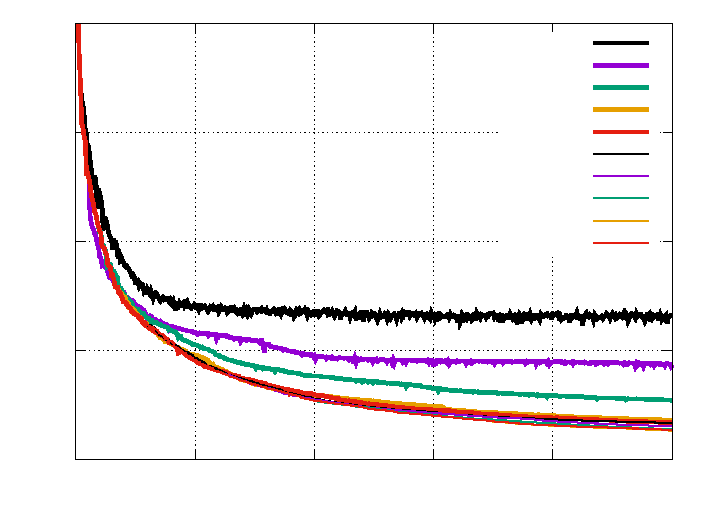
\includegraphics[width={340.00bp},height={255.00bp}]{fig}}%
    \gplfronttext
  \end{picture}%
\endgroup
}
	\caption{The } %20 polygons
	\label{foo}
\end{figure}

\begin{figure}[htbp]
	\centering
		\resizebox{.45\textwidth}{!}{% GNUPLOT: LaTeX picture with Postscript
\begingroup
  \makeatletter
  \providecommand\color[2][]{%
    \GenericError{(gnuplot) \space\space\space\@spaces}{%
      Package color not loaded in conjunction with
      terminal option `colourtext'%
    }{See the gnuplot documentation for explanation.%
    }{Either use 'blacktext' in gnuplot or load the package
      color.sty in LaTeX.}%
    \renewcommand\color[2][]{}%
  }%
  \providecommand\includegraphics[2][]{%
    \GenericError{(gnuplot) \space\space\space\@spaces}{%
      Package graphicx or graphics not loaded%
    }{See the gnuplot documentation for explanation.%
    }{The gnuplot epslatex terminal needs graphicx.sty or graphics.sty.}%
    \renewcommand\includegraphics[2][]{}%
  }%
  \providecommand\rotatebox[2]{#2}%
  \@ifundefined{ifGPcolor}{%
    \newif\ifGPcolor
    \GPcolortrue
  }{}%
  \@ifundefined{ifGPblacktext}{%
    \newif\ifGPblacktext
    \GPblacktexttrue
  }{}%
  % define a \g@addto@macro without @ in the name:
  \let\gplgaddtomacro\g@addto@macro
  % define empty templates for all commands taking text:
  \gdef\gplbacktext{}%
  \gdef\gplfronttext{}%
  \makeatother
  \ifGPblacktext
    % no textcolor at all
    \def\colorrgb#1{}%
    \def\colorgray#1{}%
  \else
    % gray or color?
    \ifGPcolor
      \def\colorrgb#1{\color[rgb]{#1}}%
      \def\colorgray#1{\color[gray]{#1}}%
      \expandafter\def\csname LTw\endcsname{\color{white}}%
      \expandafter\def\csname LTb\endcsname{\color{black}}%
      \expandafter\def\csname LTa\endcsname{\color{black}}%
      \expandafter\def\csname LT0\endcsname{\color[rgb]{1,0,0}}%
      \expandafter\def\csname LT1\endcsname{\color[rgb]{0,1,0}}%
      \expandafter\def\csname LT2\endcsname{\color[rgb]{0,0,1}}%
      \expandafter\def\csname LT3\endcsname{\color[rgb]{1,0,1}}%
      \expandafter\def\csname LT4\endcsname{\color[rgb]{0,1,1}}%
      \expandafter\def\csname LT5\endcsname{\color[rgb]{1,1,0}}%
      \expandafter\def\csname LT6\endcsname{\color[rgb]{0,0,0}}%
      \expandafter\def\csname LT7\endcsname{\color[rgb]{1,0.3,0}}%
      \expandafter\def\csname LT8\endcsname{\color[rgb]{0.5,0.5,0.5}}%
    \else
      % gray
      \def\colorrgb#1{\color{black}}%
      \def\colorgray#1{\color[gray]{#1}}%
      \expandafter\def\csname LTw\endcsname{\color{white}}%
      \expandafter\def\csname LTb\endcsname{\color{black}}%
      \expandafter\def\csname LTa\endcsname{\color{black}}%
      \expandafter\def\csname LT0\endcsname{\color{black}}%
      \expandafter\def\csname LT1\endcsname{\color{black}}%
      \expandafter\def\csname LT2\endcsname{\color{black}}%
      \expandafter\def\csname LT3\endcsname{\color{black}}%
      \expandafter\def\csname LT4\endcsname{\color{black}}%
      \expandafter\def\csname LT5\endcsname{\color{black}}%
      \expandafter\def\csname LT6\endcsname{\color{black}}%
      \expandafter\def\csname LT7\endcsname{\color{black}}%
      \expandafter\def\csname LT8\endcsname{\color{black}}%
    \fi
  \fi
    \setlength{\unitlength}{0.0500bp}%
    \ifx\gptboxheight\undefined%
      \newlength{\gptboxheight}%
      \newlength{\gptboxwidth}%
      \newsavebox{\gptboxtext}%
    \fi%
    \setlength{\fboxrule}{0.5pt}%
    \setlength{\fboxsep}{1pt}%
    \definecolor{tbcol}{rgb}{1,1,1}%
\begin{picture}(6800.00,5100.00)%
    \gplgaddtomacro\gplbacktext{%
      \csname LTb\endcsname%%
      \put(605,681){\makebox(0,0)[r]{\strut{}$0$}}%
      \csname LTb\endcsname%%
      \put(605,1727){\makebox(0,0)[r]{\strut{}$5$}}%
      \csname LTb\endcsname%%
      \put(605,2774){\makebox(0,0)[r]{\strut{}$10$}}%
      \csname LTb\endcsname%%
      \put(605,3820){\makebox(0,0)[r]{\strut{}$15$}}%
      \csname LTb\endcsname%%
      \put(605,4866){\makebox(0,0)[r]{\strut{}$20$}}%
      \csname LTb\endcsname%%
      \put(717,468){\makebox(0,0){\strut{}$0$}}%
      \csname LTb\endcsname%%
      \put(1862,468){\makebox(0,0){\strut{}$100$}}%
      \csname LTb\endcsname%%
      \put(3007,468){\makebox(0,0){\strut{}$200$}}%
      \csname LTb\endcsname%%
      \put(4153,468){\makebox(0,0){\strut{}$300$}}%
      \csname LTb\endcsname%%
      \put(5298,468){\makebox(0,0){\strut{}$400$}}%
      \csname LTb\endcsname%%
      \put(6443,468){\makebox(0,0){\strut{}$500$}}%
    }%
    \gplgaddtomacro\gplfronttext{%
      \csname LTb\endcsname%%
      \put(191,2773){\rotatebox{-270}{\makebox(0,0){\strut{}Error (\%)}}}%
      \csname LTb\endcsname%%
      \put(3580,149){\makebox(0,0){\strut{}Generation}}%
      \csname LTb\endcsname%%
      \put(5574,4674){\makebox(0,0)[r]{\strut{}$k_{max}=5$}}%
      \csname LTb\endcsname%%
      \put(5574,4461){\makebox(0,0)[r]{\strut{}$k_{max}=10$}}%
      \csname LTb\endcsname%%
      \put(5574,4248){\makebox(0,0)[r]{\strut{}$k_{max}=15$}}%
      \csname LTb\endcsname%%
      \put(5574,4035){\makebox(0,0)[r]{\strut{}$k_{max}=20$}}%
      \csname LTb\endcsname%%
      \put(5574,3822){\makebox(0,0)[r]{\strut{}$k_{max}=25$}}%
      \csname LTb\endcsname%%
      \put(5574,3609){\makebox(0,0)[r]{\strut{}$k_{max}=30$}}%
      \csname LTb\endcsname%%
      \put(5574,3396){\makebox(0,0)[r]{\strut{}$k_{max}=40$}}%
      \csname LTb\endcsname%%
      \put(5574,3183){\makebox(0,0)[r]{\strut{}$k_{max}=50$}}%
      \csname LTb\endcsname%%
      \put(5574,2970){\makebox(0,0)[r]{\strut{}$k_{max}=60$}}%
      \csname LTb\endcsname%%
      \put(5574,2757){\makebox(0,0)[r]{\strut{}$k_{max}=70$}}%
    }%
    \gplbacktext
    \put(0,0){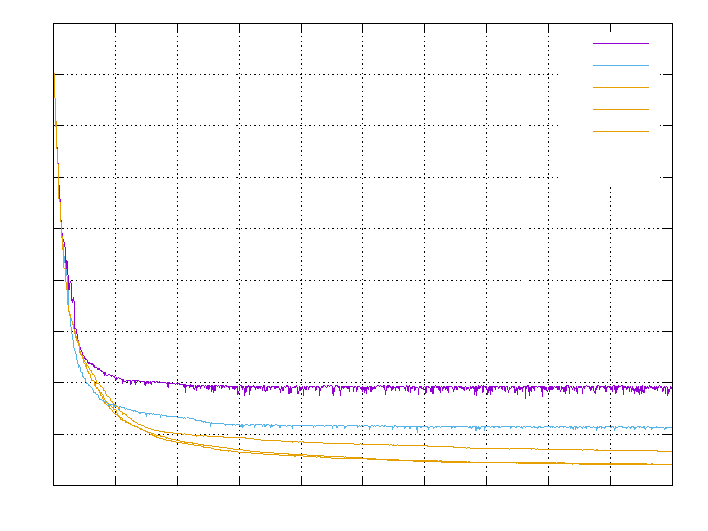
\includegraphics[width={340.00bp},height={255.00bp}]{fig_cat}}%
    \gplfronttext
  \end{picture}%
\endgroup
}
	\caption{TODO}
	\label{foo}
\end{figure}


\section{Summary}


\begin{thebibliography}{00}

\bibitem{ga-book}Sivanandam, S. N. and Deepa, S. N., ``Introduction to Genetic Algorithms'',
	Springer-Verlag Berlin Heidelberg, 2008, ISBN 978-3-540-73189-4

\bibitem{mar-io}Baldominos A., Saez Y., Recio G., Calle J. ``Learning Levels of Mario AI Using Genetic Algorithms``,
	In: Advances in Artificial Intelligence. CAEPIA 2015. Lecture Notes in Computer Science, vol 9422. Springer, Cham. doi: 10.1007/978-3-319-24598-0\_24

\bibitem{ga-transport}C. Lin, J. Yu, J. Liu and C. Lee, ``Genetic Algorithm for Shortest Driving Time in Intelligent Transportation Systems``, 2008 International Conference on Multimedia and Ubiquitous Engineering, 2008, pp. 402-406, doi: 10.1109/MUE.2008.16.

\bibitem{ga-scheduling}Lim, C., and Eoksu S., ``Production planning in manufacturing/remanufacturing environment using genetic algorithm``, Proceedings of the 7th annual conference on Genetic and evolutionary computation. 2005.

\bibitem{ga-robocode}Shichel Y., Ziserman E., Sipper M., ``Using Genetic Programming to Evolve Robocode Players`` In: Genetic Programming. EuroGP 2005. Lecture Notes in Computer Science, vol 3447. Springer, Berlin, Heidelberg. https://doi.org/10.1007/978-3-540-31989-4\_13

\bibitem{ga-portfolio}S. Slimane and M. Benbouziane, ``Portfolio Selection Using Genetic Algorithm`` In: Journal of Applied Finance \& Banking , Vol. 2, No. 4 (2012): pp. 143-154.

\bibitem{ga-trading}R.J. Kuo, C.H. Chen, Y.C. Hwang, ``An intelligent stock trading decision support system through integration of genetic algorithm based fuzzy neural network and artificial neural network``,
Fuzzy Sets and Systems,
Volume 118, Issue 1,
2001,
Pages 21-45,
ISSN 0165-0114,
10.1016/S0165-0114(98)00399-6.

\bibitem{image-proc}Jayaraman, S., S. Esakkirajan, and T. Veerakumar. ``Digital image processing``, Mc Graw Hill India, 2009, ISBN 978-0070144798

%\bibitem{b2}ISO 516:2019. Camera shutters — Timing — General definition and
%	mechanical shutter measurements. International Organization for Standardization,
%	2019. Online: https://www.iso.org/obp/ui/\#iso:std:iso:516:ed-4:v1:en
%
%\bibitem{b3}Y. Asakura, et al., ``Exposure precision tester and exposure precision
%	testing method for camera'', U.S. Patent 5 895 132, Apr. 20, 1999.
%
%\bibitem{b4}Peter D. Hiscocks, ``Measuring Camera Shutter Speed'',
%	Royal Astronomical Society, Toronto Centre, Canada, 2010.
%	Online: https://www.ee.ryerson.ca/~phiscock/astronomy/light-pollution/shutter-cal.pdf
%
%\bibitem{b5}V. N. Budilov, V. I. Volovach, M. V. Shakurskiy and S. V. Eliseeva,
%``Automated measurement of digital video cameras exposure time'',
%	East-West Design \& Test Symposium (EWDTS 2013), Rostov-on-Don,
%	2013, pp. 1-4. doi: 10.1109/EWDTS.2013.6673136
%
%
%\bibitem{b6}CCTVCAD Lab Toolkit. CCTVCAD Software. Perm, Russia, 2011.
%Online: http://www.cctvcad.com/labtoolkit\_help
%
%\bibitem{b7}L. Masson, F. Cao, C. Viard, and F. Guichard,
%	``Device and algorithms for camera timing evaluation''
%	in Proc. IS\&T/SPIE Electronic Imaging Symposium,
%	San Francisco, California, United States, 2014.
%	doi:10.1117/12.2042161
%
%\bibitem{b8}Image Engineering: LED-Panel.
%	Online: https://www.image-engineering.de/products/equipment/measurement-devices/900-led-panel
%
%\bibitem{b9}G. Shize, S. Shenghe and Z. Zhongting,
%	``A novel equivalent sampling method using in the digital storage oscilloscopes''
%	in Proc. 1994 IEEE Instrumentation and Measurement Technology Conference,
%	Hamamatsu, Japan, 1994, pp. 530-532 vol.2.
%	doi: 10.1109/IMTC.1994.351901
%
%\bibitem{b10}A. G. J. Holt, J. J. Hill and R. Linggard,
%	``Integral sampling'',
%	in Proceedings of the IEEE, vol. 61, no. 5, pp. 679-680, May 1973.
%	doi: 10.1109/PROC.1973.9138
%
%\bibitem{b11}FLIR Machine Vision Cameras.
%	Online: https://www.flir.com/browse/industrial/machine-vision-cameras/

\end{thebibliography}

\end{document}
